\tikzstyle{end} = [circle, minimum size = 0.6cm, draw, inner sep = 0.1pt]
\tikzstyle{leaf} = [circle, minimum size = 0.6cm, draw, inner sep = 0.1pt, blue]
            
\tikzstyle{level 1}=[level distance = 1.5cm, sibling distance = 2cm]
\tikzstyle{level 2}=[sibling distance = 2cm]
\tikzstyle{level 3}=[sibling distance = 1cm]
    
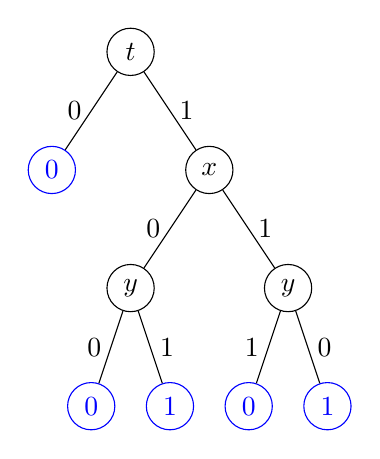
\begin{tikzpicture}[label distance=8mm]
	\node [end] (z){$t$}
       	child {
        	node[leaf] (b) {$0$}
           	edge from parent
            node[left] {$0$}
        }
        child {
        	node[end] (b) {$x$}
           	child {
               	node[end] {$y$}
               	child {
	               	node[leaf] {$0$}
	                edge from parent
		            node[left] {$0$}
	            }
			    child {
	               	node[leaf] {$1$}
	                edge from parent
		            node[right] {$1$}
	            }
                edge from parent
	            node[left] {$0$}
            }
            child {
               	node[end] {$y$}
               	child {
	               	node[leaf] {$0$}
	                edge from parent
		            node[left] {$1$}
	            }
			    child {
	               	node[leaf] {$1$}
	                edge from parent
		            node[right] {$0$}
	            }
                edge from parent
	            node[right] {$1$}
            }
           	edge from parent
            node[right] {$1$}
        };
\end{tikzpicture}

%%% Local Variables: 
%%% mode: latex
%%% TeX-master: t
%%% End: 
